\documentclass{../lab}

\labacronym{JOS}
\labtitle{Josephson Junction}

%\newcommand{\TheJosephsonEffects}{http://physics111.lib.berkeley.edu/Physics111/Reprints/JOS/04-The_Josephson_Effects.pdf}
%\newcommand{\FourWireMeasurement}{http://physics111.lib.berkeley.edu/Physics111/Reprints/JOS/10-Four_Wire_Measurement.pdf}
%\newcommand{\Physics111LibrarySite}{http://physics111.lib.berkeley.edu/Physics111/Reprints/JOS/JOS_index.html}
%\newcommand{\}{http://experimentationlab.berkeley.edu/sites/default/files/images/JOS5.gif}
%\newcommand{\}{http://experimentationlab.berkeley.edu/sites/default/files/images/JOS14.gif}
%\newcommand{\powermete}{http://experimentationlab.berkeley.edu/sites/default/files/JOS/image.jpeg}
%\newcommand{\vice}{http://experimentationlab.berkeley.edu/sites/default/files/JOS/vicepen_0.jpeg}
%\newcommand{\}{http://experimentationlab.berkeley.edu/sites/default/files/images/JOS11b.gif}

\begin{document}

\maketitle

\tableofcontents

\section{Josephson Junction Description (JOS)}

\begin{enumerate}
    \item \textbf{Note that there is NO eating or drinking in the 111-Lab anywhere, except in rooms 282 \& 286 LeConte on the bench with the BLUE stripe around it.} Thank You the Staff.
\end{enumerate}

Superconducting phenomena are among the most fascinating features in physics, and the Josephson effect is the most interesting of all. In 1962, Brian Josephson predicted that electron pairs could tunnel without resistance through an insulating barrier between two superconductors. Here we use a point contact between niobium wire with a thin oxide layer and a niobium block. Both the DC and AC Josephson effects are observed and measured. A DC current can flow through the junction with no potential difference, but when a DC voltage is applied together with a small alternating voltage, the $I$-$V$ curve shows a characteristic step structure. From this step structure the value of 2$e/h$ can be calculated easily and accurately, an exciting consequence of the properties of the junction. The ratio e/h appears throughout atomic and condensed matter physics.

In this experiment you will learn some low temperature techniques which are used in many research laboratories. You will also learn some practical and often frustrating electronics, together with manual skills in making niobium points and adjusting them to produce a useful electronic signal.

\begin{enumerate}
    \item Pre-requisites: Physics 137A (may be taken concurrently)

    \item Days Alloted for the Experiment: 8
\end{enumerate}

\textbf{All pages in this lab. Note To print Full Lab Write-up click on each link below and print separately }

I. \textbf{Josephson Junction}

II. \href{http://experimentationlab.berkeley.edu/node/104}{\textbf{How to use the digital oscilloscope}}

This lab will be graded 40\% on theory, 40\% on technique, and 20\% on analysis. For more information, see the \href{\AdvancedLabSyllabus}{\textbf{Advanced Lab Syllabus}}.

Comments: E-mail \href{\MailDonOrlando}{\textbf{Don Orlando}}

\section{Josephson Effect Photos}

\noindent
\href{http://experimentationlab.berkeley.edu/sites/default/files/images/JOS_3507.jpg}{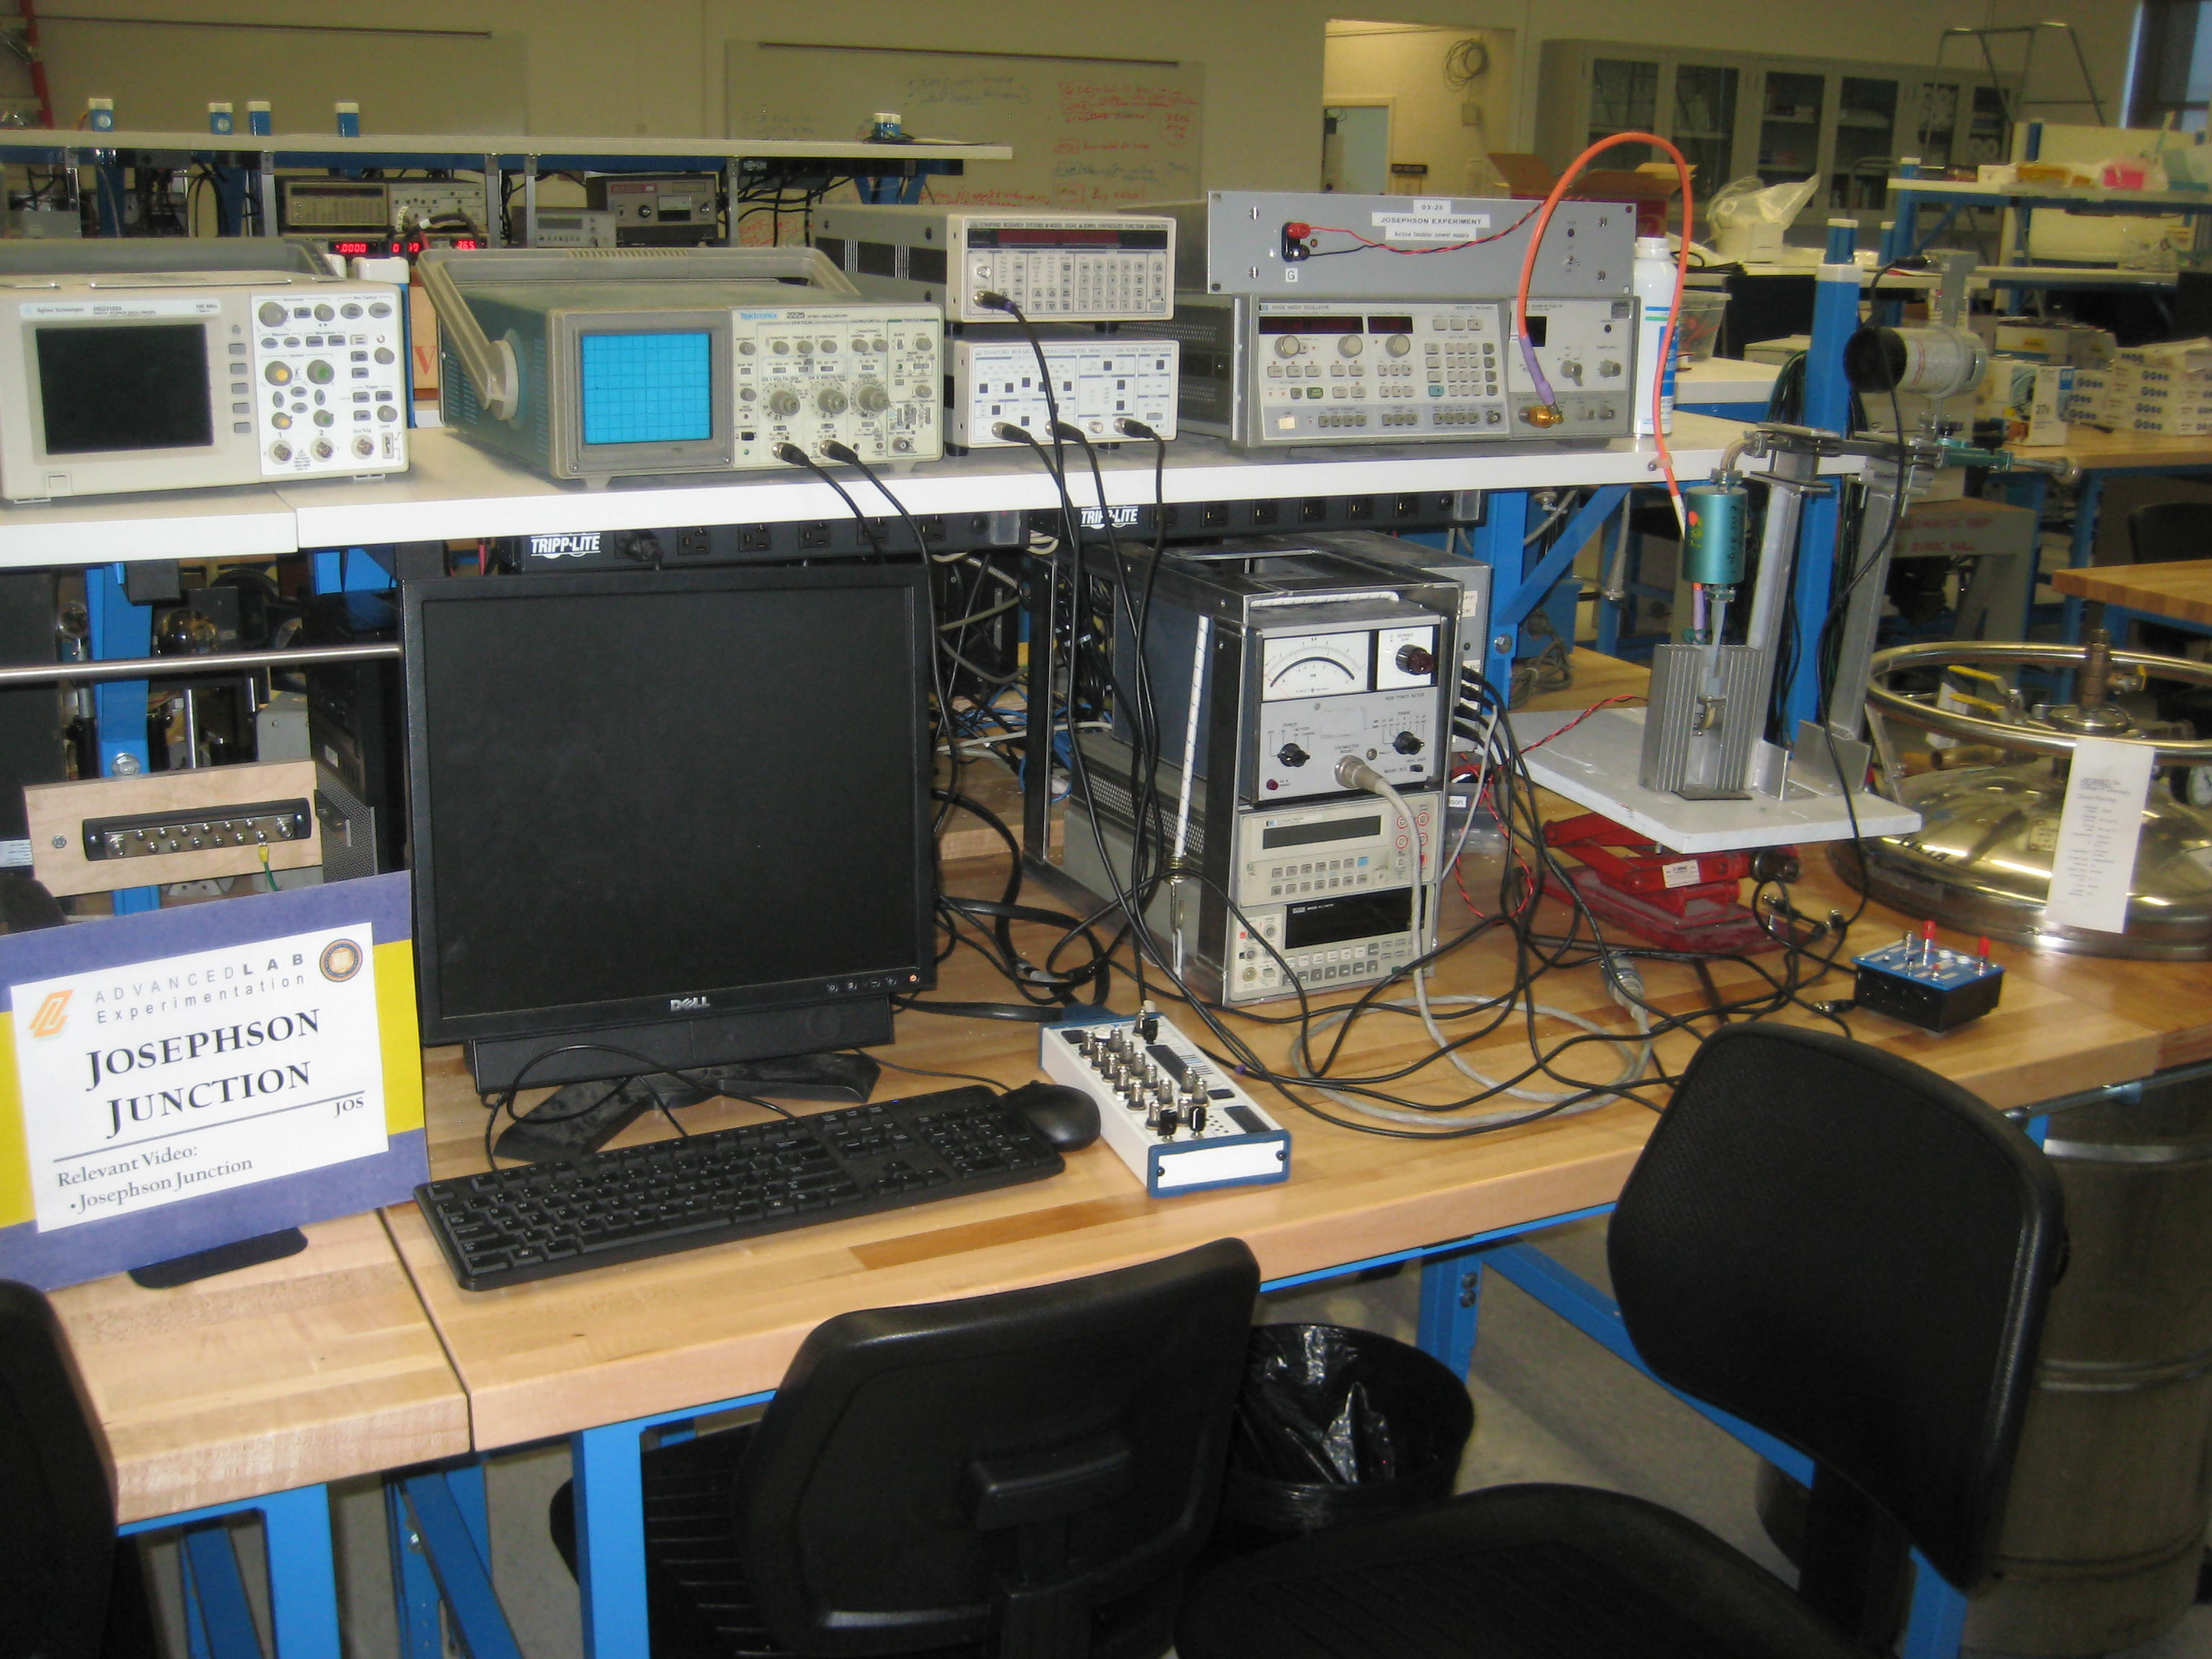
\includegraphics[width=0.25\linewidth,keepaspectratio]{images/JOS_3507.jpg}}
\href{http://experimentationlab.berkeley.edu/sites/default/files/images/JOS-Dewar_3508.jpg}{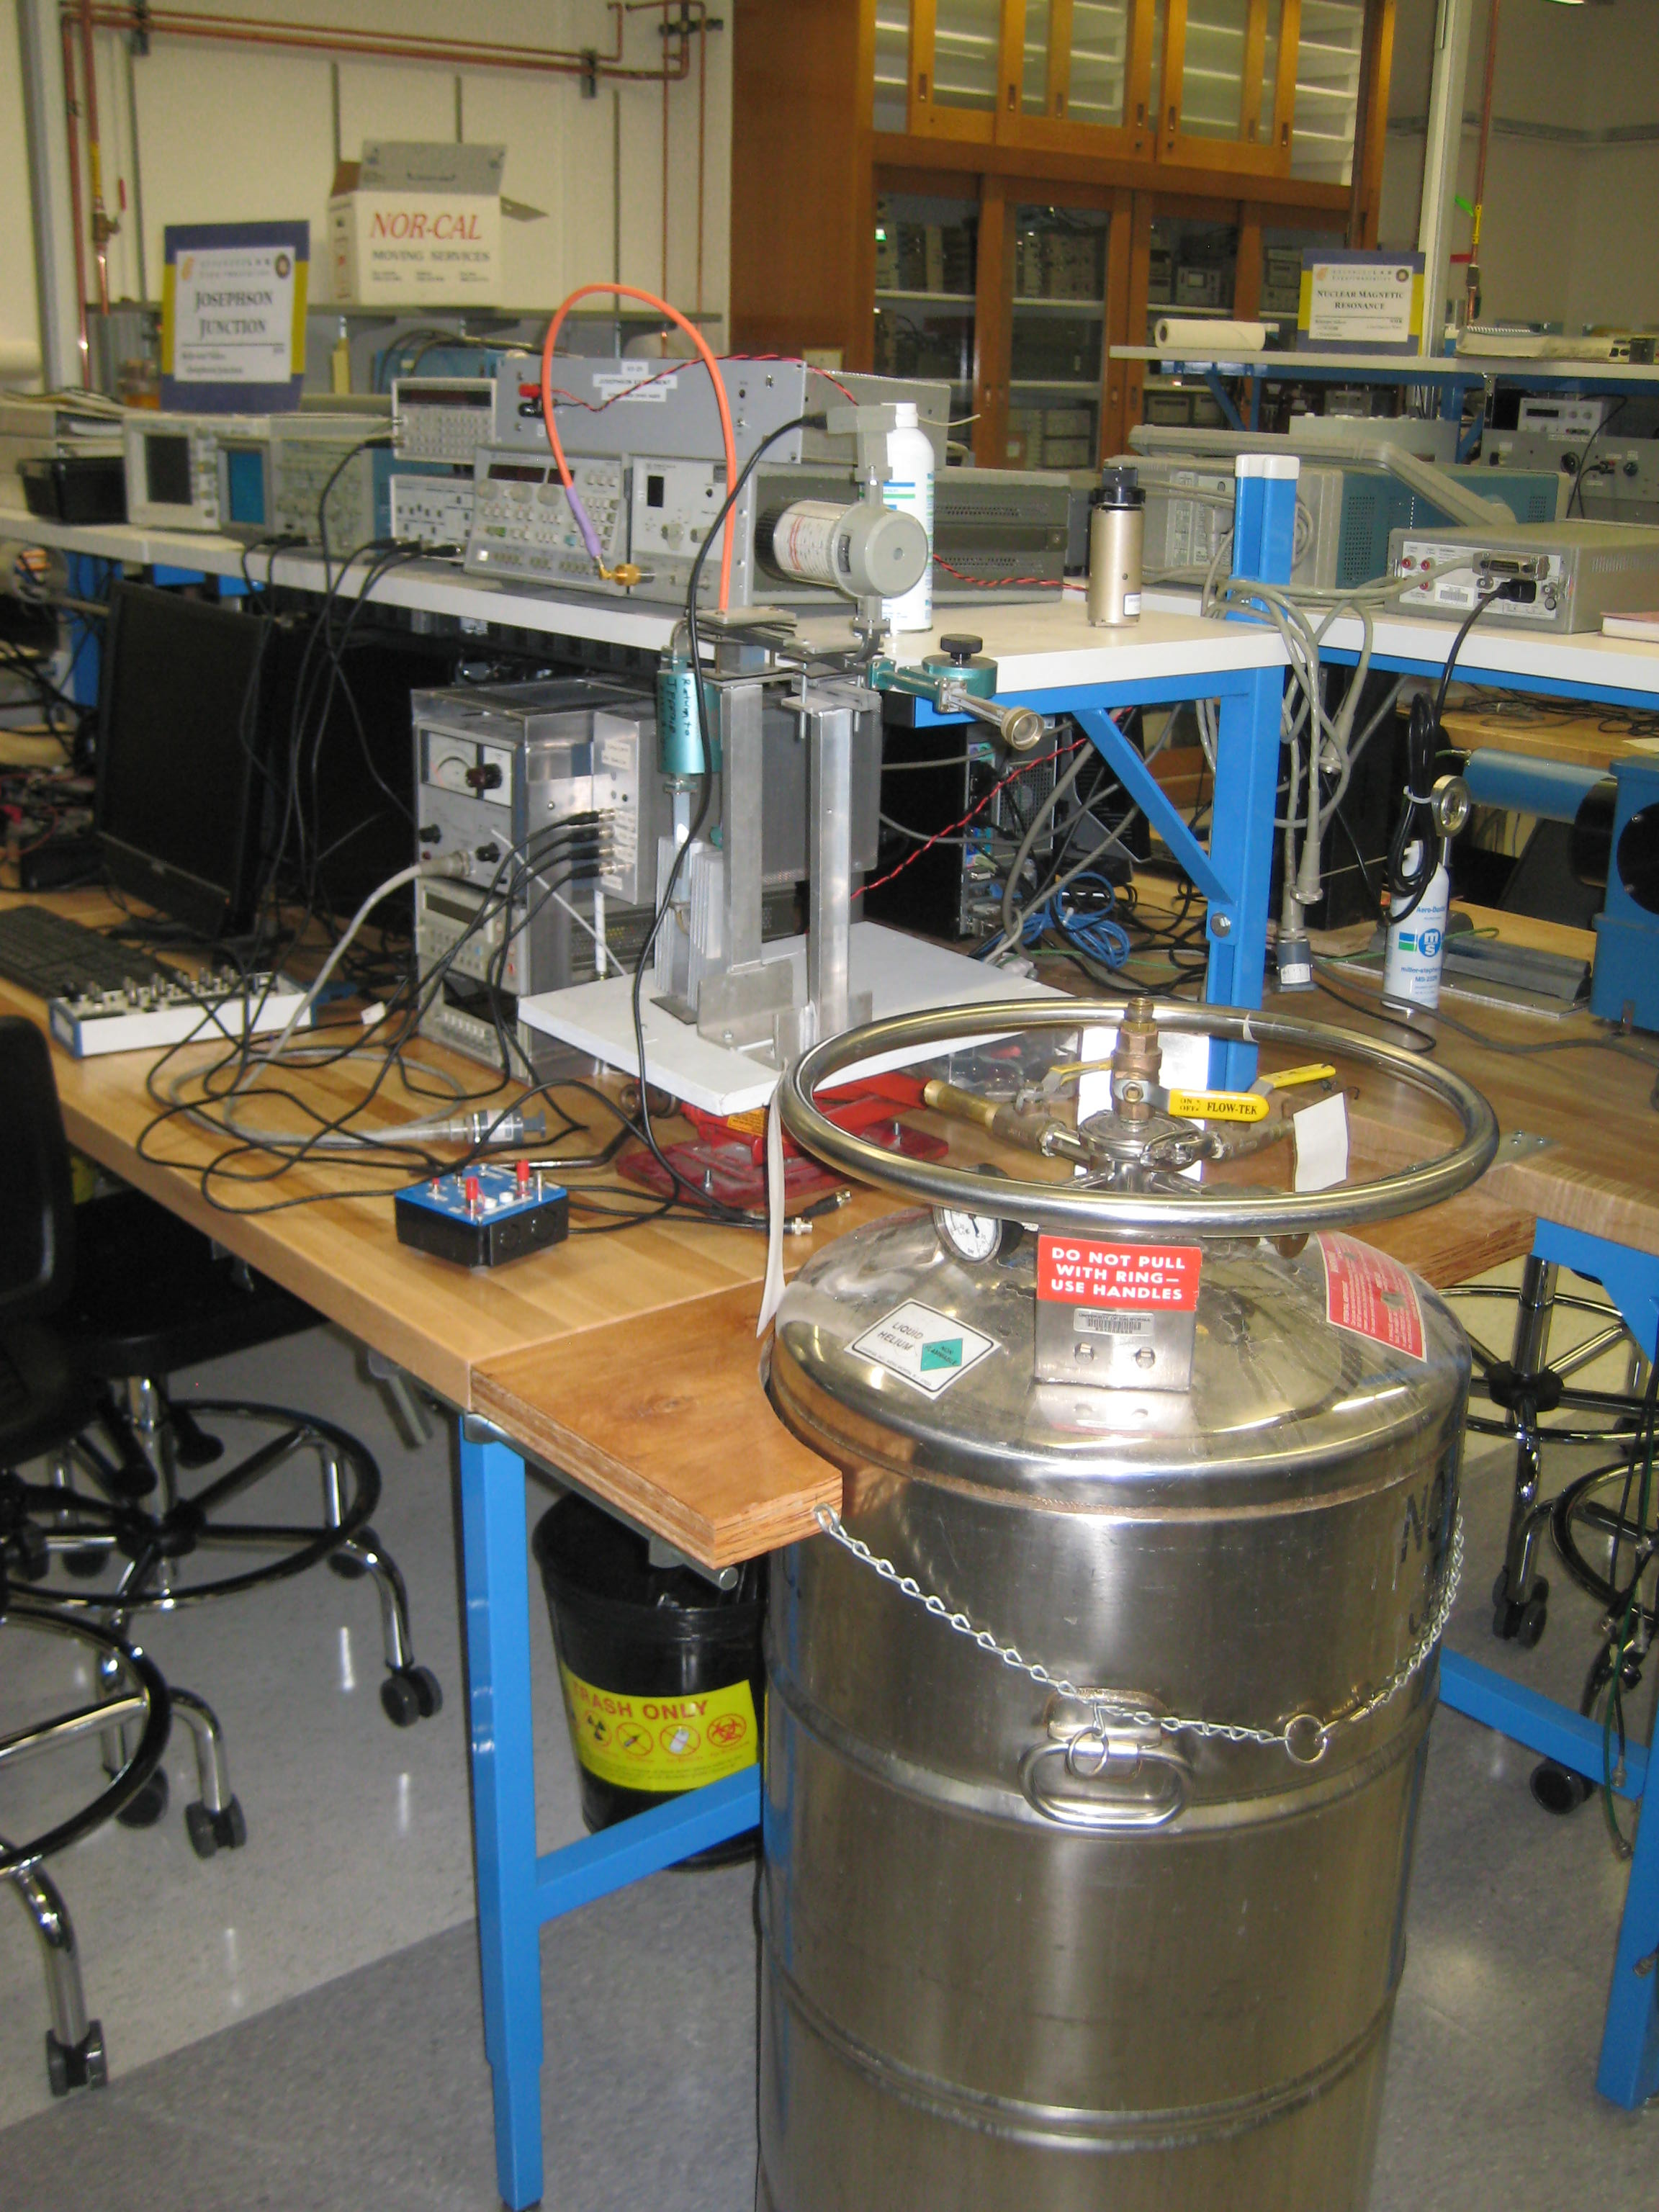
\includegraphics[width=0.25\linewidth,keepaspectratio]{images/JOS-Dewar_3508.jpg}}
\href{http://experimentationlab.berkeley.edu/sites/default/files/images/JOS-Probes_3506.jpg}{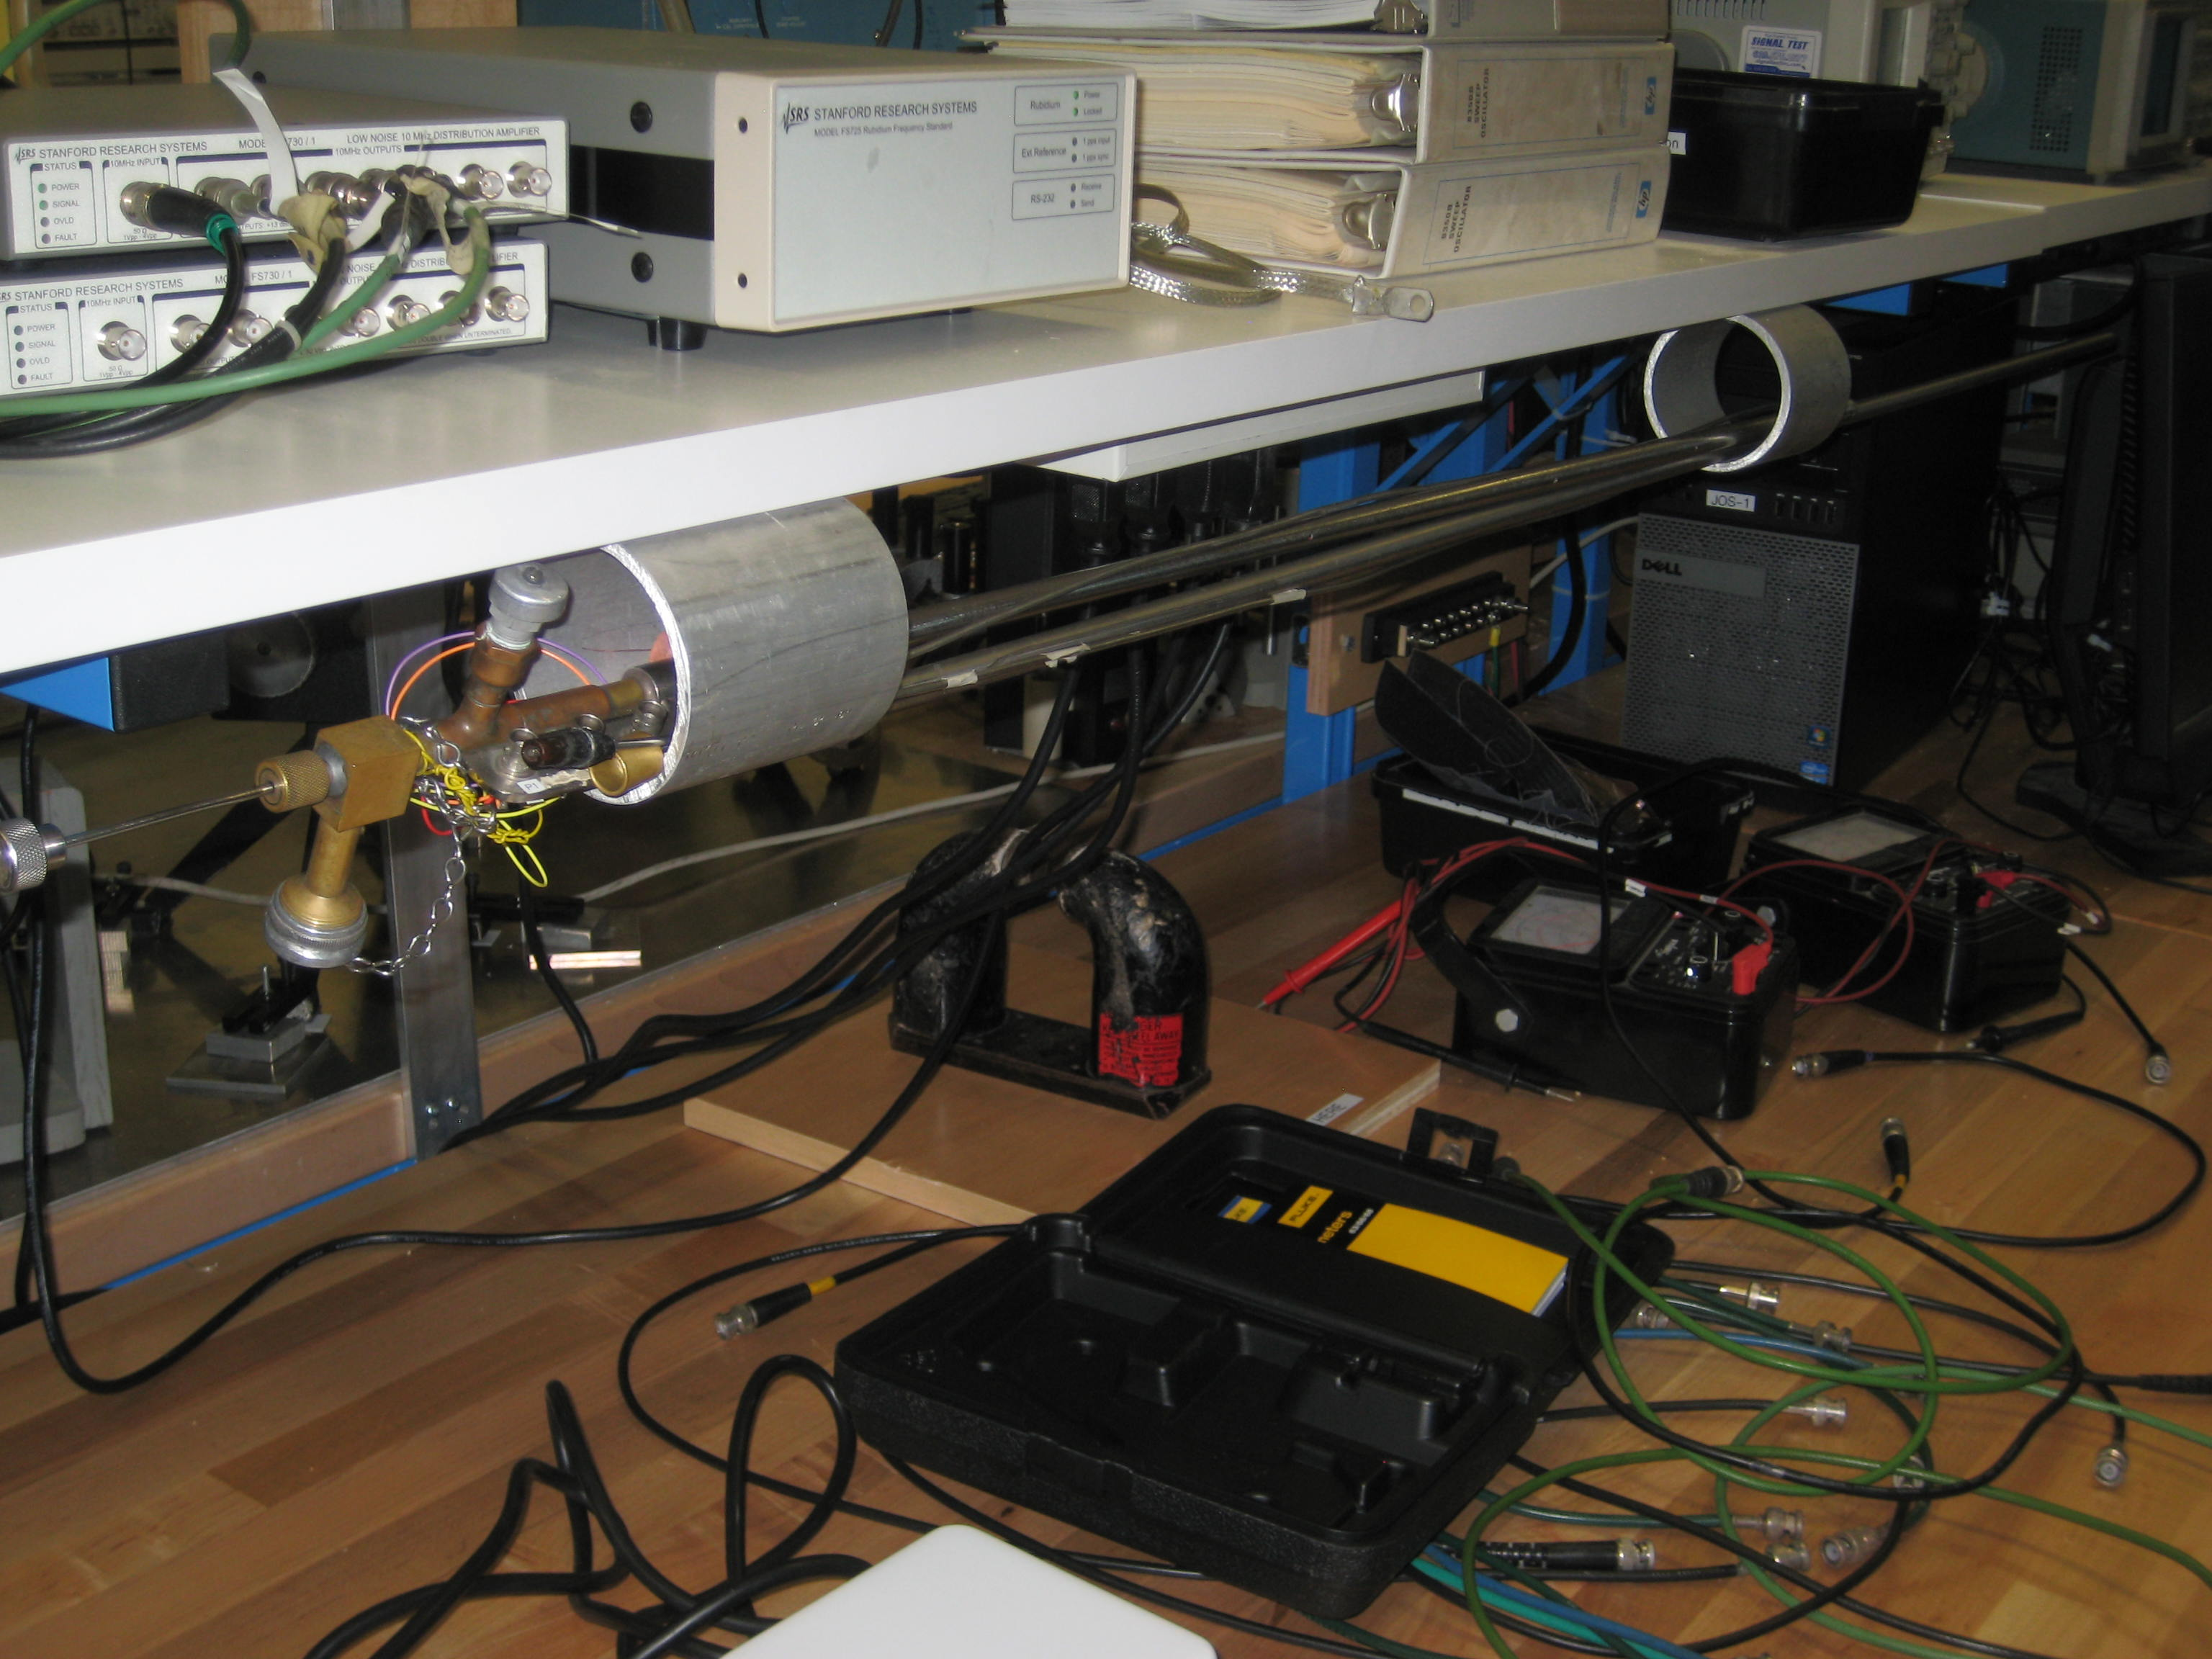
\includegraphics[width=0.25\linewidth,keepaspectratio]{images/JOS-Probes_3506.jpg}}
\href{http://experimentationlab.berkeley.edu/sites/default/files/images/HotPlate-JOS_3505-Lg.jpg}{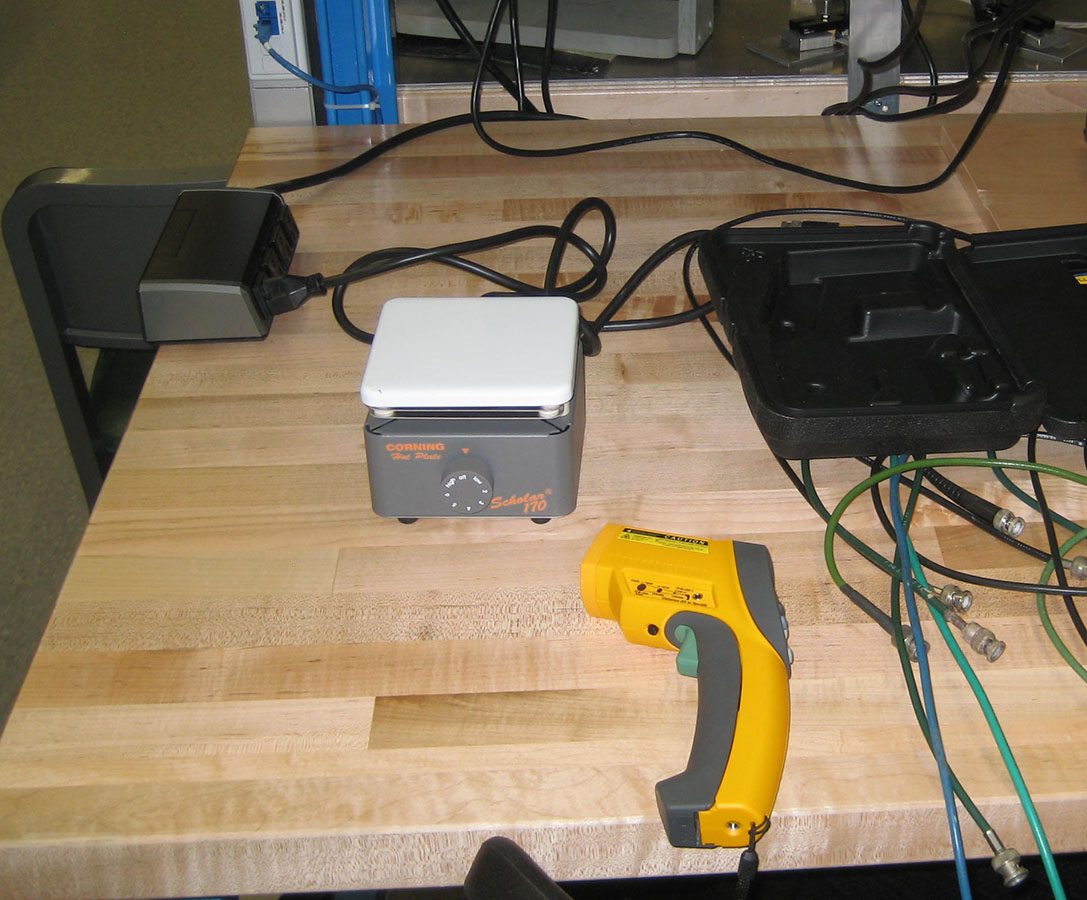
\includegraphics[width=0.25\linewidth,keepaspectratio]{images/HotPlate-JOS_3505-Lg.jpg}}

\section{Before the 1st Day of Lab}

\textbf{Complete the following before your experiment's scheduled start date:}

\begin{enumerate}
    \item View the \href{http://youtu.be/Z9vBPQrG0U4}{\textbf{Josephson Junction video}}.

    \item Complete the \href{http://experimentationlab.berkeley.edu/JOSPreLab}{\textbf{JOS Pre Lab and Evaluation}} sheets. Print, fill it out, then turn in your answers with the report. The Pre-Lab must be printed separately. Discuss the experiment and pre-lab questions with any faculty member or GSI and get it signed off by that faculty member or GSI. Turn in the signed pre-lab sheet with your lab report.

    \item Read before handling of Cryogenics: Read the Cryogenic Liquids information from the campus Environmental Health and Safety (EH\&S) department \href{http://experimentationlab.berkeley.edu/sites/default/files/SHE/77cryogenic.pdf}{\textbf{Cryogenic Liquids}}.

    \item Notify the staff/GSI to fill the liquid helium tank one (1) day before you begin the experiment.

    \item \textbf{Check points} are examination points that are placed in this lab where you must \textbf{STOP} and call a GSI or professor to make sure you understand what's expected. There could  be multiple check points throughout your lab so make sure you don't skip them since there is a \href{http://experimentationlab.berkeley.edu/checkpointjso}{\textbf{\textbf{sign off sheet}}} that must be turned in with your lab report. There are 3 Checkpoints in this lab.

\end{enumerate}

\noindent\textbf{Suggested Reading:}

\begin{enumerate}
    \item †Clarke, John, ``\href{http://physics111.lib.berkeley.edu/Physics111/Reprints/JOS/Clark_Josephson_effect_andeh.pdf}{\textbf{The Josephson Effect and e/h}},'' American Journal of Physics, Vol. 38, No. 9, September 1970, pp. 1071-1095. \href{http://physics111.lib.berkeley.edu/Physics111/Reprints/JOS/03-The\_Josephson\_Effect\_and\_e\_h.pdf}{\textbf{Searchable Page}}

    \item †Feynman, R.P., Leighton, R.B., and Sands, M. \href{http://physics111.lib.berkeley.edu/Physics111/Reprints/JOS/08-Superconductivity.pdf}{\textbf{The Feynman Lectures on Physics}}.. Vol. III. Menlo Park: Addison-Wesley, 1966.

    \item †Langenberg, D.N., Scalapion, D.J., and Taylor, B.N. ``\href{http://physics111.lib.berkeley.edu/Physics111/Reprints/JOS/04-The\_Josephson\_Effects.pdf}{\textbf{The Josephson Effects}},'' Scientific American, Vol.214, p.30, May, 1966. Published article \href{http://prola.aps.org/abstract/PR/v150/i1/p186\_1}{\textbf{APS site}}

    \item †Richards, P.I., Shapiro, S., and Grimes, C.C. ``\href{http://physics111.lib.berkeley.edu/Physics111/Reprints/JOS/01-Student_Laboratory_Demonstration.pdf}{\textbf{Student Laboratory Demonstration of Flux Quantization and the Josephson Effect in Superconductors}},'' American Journal of Physics, Vol. 36, No. 8, August 1968, pp. 690-697. \href{http://physics111.lib.berkeley.edu/Physics111/Reprints/JOS/01-Student\_Laboratory\_Demonstration.pdf}{\textbf{Searchable Page}}

    \item Anderson, Philip W. ``\href{http://physics111.lib.berkeley.edu/Physics111/Reprints/JOS/05-How_Josephson_Discovered_his_Effect.pdf}{\textbf{How Josephson Discovered His Effect}}''; Physics Today: November, 1970, pp. 23-29. (PAGES 26 \& 28 ARE INTENTIONALLY MISSING.)

    \item \href{http://physics111.lib.berkeley.edu/Physics111/Reprints/JOS/10-Four\_Wire\_Measurement.pdf}{\textbf{Four Wire Measurements}}

    \item \href{http://physics111.lib.berkeley.edu/Physics111/Reprints/JOS/JOS\_index.html}{\textbf{Josephson Reprints}}on Physics 111-Lab Library site

    \item Last day of the experiment please fill out the \href{\ExperimentEvaluation}{\textbf{Experiment Evaluation}}

\end{enumerate}

More \hyperref[sec:References]{References}

You should keep a laboratory notebook. The notebook should contain a detailed record of everything that was done and how/why it was done, as well as all of the data and analysis, also with plenty of how/why entries. This will aid you when you write your report.

\section{Objectives}

\begin{itemize}
    \item Learn what real experimental physics is about

    \item Learn the synergy between experimental and theoretical work

    \item Learn to use pieces of equipment that are commonly used in research

    \item Learn how measurements are performed, analyzed, and interpreted.

    \item Learn how to present your work and results

    \item Learn problem solving strategies

    \item Learn how to manage and organize your time

    \item Understand what is superconductivity and how it relates to the Josephson Junction effect.

    \item Deeply explore and understand what are the DC and AC Josephson effect.

    \item Learn how the experiment works and how to use the equipment properly as well as mastering the experiment's procedure.

    \item Analyze any data you take and argue why does that data make sense or doesn't.(Demonstrate the steps you take to get to these conclusions.)

\end{itemize}

\section{Intent and scope of this laboratory manual}

This manual is intended to provide general guidance for the lab. It is \emph{not} designed to explain all the physics necessary for understanding this experiment. Nor is it a ``cook-book'' telling you exactly which buttons to press, etc. It is up to the student to become familiar with the necessary material in the reprints, and to figure out the exact procedure necessary for completion of the assignments in the lab. Talk with an instructor often, but not until you have given the physics and procedures some thought first. We are here to instruct and help, but not to do your thinking for you.

\section{Introduction}

In this experiment you will construct a Josephson junction, use it to observe the DC and AC Josephson effects, and measure the ratio of fundamental constants
\begin{equation}
    \frac{2e}{h} \cong 483.60 \textrm{ MHz}/\mu \textrm{V}
\end{equation}
You will learn the techniques in Low Temperature four wire measurements and handling Liquid Helium.

\section{Apparatus}

\subsection{The junction}

The central component of this experiment is the point-contact junction (PCJ), shown in Figure \ref{fig:junction}. It is a niobium needle that is delicately pressed against a niobium screw. Both pieces have oxide layers that form a barrier to electrical conduction between the niobium pieces. The thin oxide layers and the small contact area between the needle's point and the screw provide the \emph{weak-link} necessary to observe Josephson tunneling.

\begin{figure}[h]
    \centering
    \href{http://experimentationlab.berkeley.edu/sites/default/files/images/JOS4.gif}{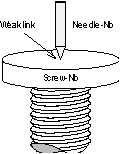
\includegraphics[width=0.3\linewidth]{images/JOS4.png}}
    \caption{The Junction}
    \label{fig:junction}
\end{figure}

\subsection{The junction assembly}

The junction is mounted in an assembly shown in Figure \ref{fig:JunctionAssemblyDiagram}. To adjust the pressure in the junction, we use a mechanism called a \emph{differential screw }(D)\emph{,} which moves the niobium needle point towards the niobium base screw (FB) with a great deal of control. The needle (A) fits into a hole in a form (B) made of a kind of fiberglass called ``G10.'' The needle is held in place by two screws (not shown in Figure \ref{fig:JunctionAssemblyDiagram} [see Figure \ref{fig:DetailsOfPointHolderConstruction}]). The body piece (B) can slide up and down on the two stainless steel rods (C). The flat base (FB) of the junction is held rigidly in place in G10 and cannot slide up or down. The differential screw (D) has pitch of 72 threads per inch at the top and a pitch of 80 threads per inch at the tip fixed in (B).

When the differential screw (D) is advanced one turn, it moves down 1/72''. But part (B), which cannot rotate, moves up 1/80''. The net motion of the needle with respect to the Nb base is thus only 1/720'' (= 1/72'' - 1/80''). Even with this effective pitch of 720 turns per inch, the screw must be turned \emph{very slowly} to prevent damaging the needle point.

\begin{figure}[h]
    \centering
    \href{http://experimentationlab.berkeley.edu/sites/default/files/images/JOS5.gif}{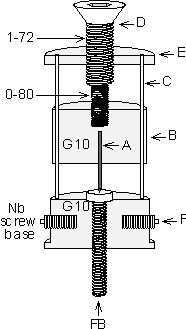
\includegraphics[width=0.4\linewidth]{images/JOS5.png}}
    \caption{Junction Assembly}
    \label{fig:JunctionAssemblyDiagram}
\end{figure}

\subsection{The Cryogenic Probe assembly}

The junction assembly is mounted in a \emph{probe}, manufactured from a $\sim$three foot length of 1/2" diameter Stainless Steel Tubing (SST), as shown in Figure \ref{fig:probe}. This tube serves as a holder for the junction assembly and as a waveguide for the microwaves used in the observation of the AC effect.

The junction end of the probe is inserted into a cryostat filled with liquid helium. The other end remains outside the cryostat and provides the electrical connections (not shown), radio-frequency (RF) coupling port, and differential screw manipulator (labeled \emph{Hand adjustment}). The junction is held in the probe by set screws (F). When the screws are turned counterclockwise (advancing them outward), the screw heads engage in a retaining hole in the SST wall, locking the assembly in place. (Note that as the screw holes in the assembly were not drilled 180 degrees apart, while the retaining holes were, both set screws cannot be engaged simultaneously. One screw goes through a retaining hole, the other can be adjusted to keep the fit secure.)

\begin{figure}[h]
    \centering
    \href{http://experimentationlab.berkeley.edu/sites/default/files/images/JOS6.jpg}{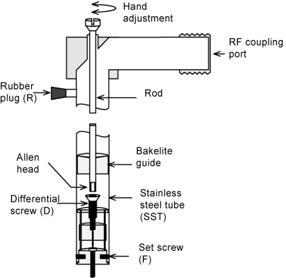
\includegraphics[width=0.5\linewidth]{images/JOS6.jpg}}
    \caption{The Probe}
    \label{fig:probe}
\end{figure}

\subsection{\texorpdfstring{$I$-$V$}{I-V} Measurements}

All of your measurements will be made by examining the current-voltage ($I$-$V$) characteristic of the junction. The $I$-$V$ curve is traced by measuring the voltage that develops across the junction as the current is swept by a low frequency ($\sim$60 Hz) oscillator \href{https://youtu.be/PrM8DHFOFS0}{\textbf{SRS DS 345}}. Since the impedance of the junction is small, a standard four-terminal measurement must be used. \href{http://physics111.lib.berkeley.edu/Physics111/Reprints/JOS/10-Four\_Wire\_Measurement.pdf}{\textbf{Four Wire Measurement}}. \textbf{This is a very important way of measurement for this experiment}. You will get a resistive measurement instead of a $I/V$ curve measurement.

The electronic hookup is shown in Figure \ref{fig:ElectronicsBlockDiagram}. The parts in the dashed area are physically located below in the  \href{http://experimentationlab.berkeley.edu/sites/default/files/JOS/image.jpeg}{\textbf{small gray box}} next to the power meter. The four electrical connections to the junction are labeled P1, P2, and B1, B2 on the side of the box.

\begin{figure}[h]
    \href{http://experimentationlab.berkeley.edu/sites/default/files/images/JOS7.gif}{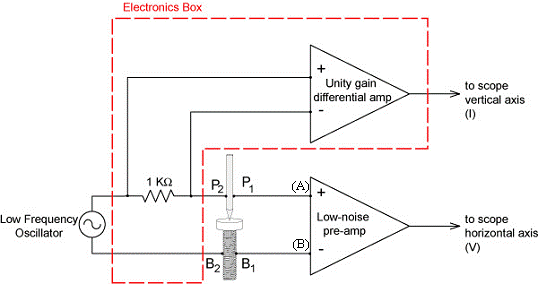
\includegraphics[width=0.6\linewidth]{images/JOS7.png}}\hfill
    \href{http://experimentationlab.berkeley.edu/sites/default/files/JOS/image.jpeg}{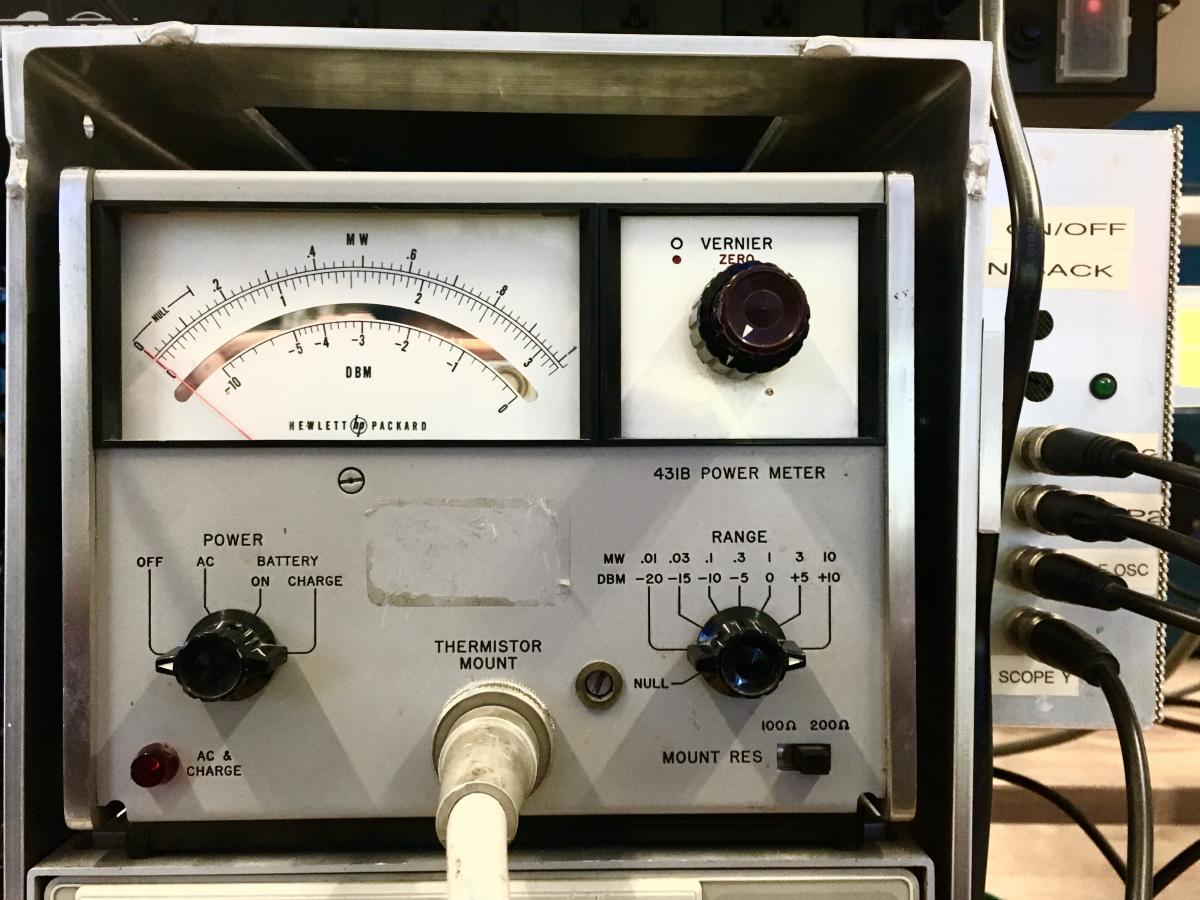
\includegraphics[width=0.39\linewidth]{images/image.jpg}}
    \caption{Electronics Block Diagram}
    \label{fig:ElectronicsBlockDiagram}
\end{figure}

\subsection{The Radio-Frequency electromagnetic radiation (RF)}

The RF is generated by a Hewlett-Packard model 8350B \emph{sweep oscillator} running in continuous-wave (CW) mode, outputting maximum power of $\sim$20 dBm. The oscillator output is connected to an \emph{active doubler}, a semiconductor device which amplifies the output by $\sim$20 dBm (up to a maximum of $\sim$29 dBm) and doubles the frequency. For example, setting the HP to 11 GHz and 5 dBm will result in $\sim$25 dBm of 22 GHz RF out of the doubler. The doubler is mounted to a heat sink and to the wave guide. The wave guide connects through an isolator, a power splitter (\emph{directional coupler}), an attenuator, and finally to the cryogenic probe. The isolator prevents potentially damaging reflections from returning to the doubler. The power splitter picks off a fraction of the RF power and sends it to an RF frequency measurement instrument consisting of a variably-tuned absorption cavity and a crystal RF power detector. The output of the crystal detector is an electrical signal that is proportional to the RF power incident on the detector. RF frequency measurement is achieved by tuning the absorption cavity until a reduction in the magnitude of the detector output is observed on the oscilloscope. The frequency is then read off the graduated scale on the absorption cavity. Its accuracy is much better than that of the RF source.

\begin{figure}[h]
    \centering
    \href{http://experimentationlab.berkeley.edu/sites/default/files/images/JOS9.jpg}{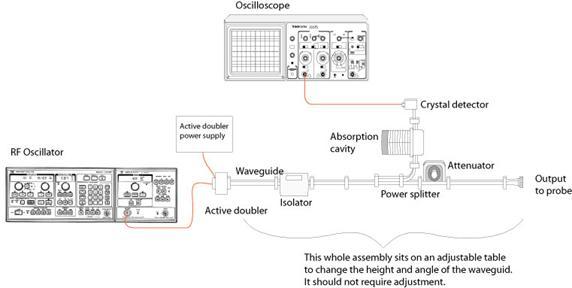
\includegraphics[width=0.7\linewidth]{images/JOS9.jpg}}
    \caption{The RF Equipment}
    \label{fig:RFEquipment}
\end{figure}

\section{Cryogenics Safety}

The liquid helium is contained in a $\sim$5 foot tall insulated vessel called a \emph{cryostat}. You must notify the lab staff at least once day in advance that you will need liquid helium for your lab and before it is near empty (about 4 liters remaining).

\textbf{Read before handling of Cryogenics: Read the Cryogenic Liquids information from the campus Environmental Health and Safety (EH\&S) department } \href{http://experimentationlab.berkeley.edu/sites/default/files/images/77cryogenic.pdf}{\textbf{Cryogenic Liquids}}

\begin{figure}[h]
    \centering
    \href{http://experimentationlab.berkeley.edu/sites/default/files/images/JOS10.gif}{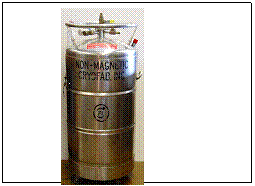
\includegraphics[width=0.4\linewidth]{images/JOS10.png}}
    \caption{}
    \label{fig:JOS10}
\end{figure}

\section{Procedure}

\subsection{Prep and Clean-up}

There are many little parts and tools associated with the apparatus. You must keep the area clean! When you leave for the day, assemble the probe and put it back in its holder, get the cables off of the floor, and collect the tools. Keeping the area clean and organized will not only save you a great deal of time but also will serve you as practice when working in future experiments that involve a whole lot of equipment.

\subsection{Making a point}

Grab a pair disposable gloves to avoid any extra impurities on the Nb tip.Take a short Nb wire (around 5/8 of an inch long) and shape it with a file (See GSI or professor to cut for you 6 Inches of Nb wire). It is best to use the \href{http://experimentationlab.berkeley.edu/sites/default/files/JOS/vicepen\_0.jpeg}{\textbf{pen vice}} at your station to hold the point. File evenly around the point by rotating the vise so you get a conical shape, with sides at roughly 45 degrees to the axis of the point. (Significantly smaller angles will weaken the point, while significantly larger angles may make for a messy contact.) After shaping it with the file, smooth the surface of the tip with emery paper, or fine sandpaper. (There should be a variety of grades of sand paper under the table.) Check the appearance of the point by eye or with a microscope. The appearance should be something like Figure \ref{fig:NbTipMagnification}. Holding the point over a white surface, like a sheet of paper, can make it easier to see its shape.

\begin{figure}[h]
    \centering
    \href{http://experimentationlab.berkeley.edu/sites/default/files/images/250px-JOS11b.gif}{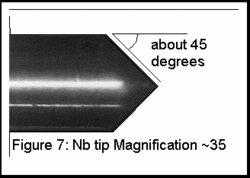
\includegraphics[width=0.5\linewidth]{images/250px-JOS11b.png}}
    \caption{Nb Tip Magnification}
    \label{fig:NbTipMagnification}
\end{figure}
 
By far the best results are obtained by leaving the point out in air to oxidize overnight. You can get a working point right away by using a hot plate, but it is extremely difficult to get the desired amount of oxidation and avoid introducing impurities. If you absolutely need a working point right away, preheat the hot plate. Then put your point on the plate for approximately 25 seconds to a minute, or until the point achieves a nice brassy color. Don't have high expectations for this hot plate point, though.

It is recommended that you spend the first day of this experiment making the points that you will use in the succeeding days. You should make at least five right away. Once you've done this, take some time to familiarize yourself with the equipment; you don't have to take data your first day. Make sure that once your done with your experiment you throw your tips away, you don't want someone else to benefit from your hard work while they do nothing.

\subsection{Remove the junction assembly from the probe}

This is the most delicate part of the lab. Please work over a clean surface, exercise caution, use your good judgment, and consult the lab staff if you have any uncertainty about what to do. Please refer to Figure 2, repeated here for your reference, as well as photographs of the junction assembly in Figure \ref{fig:JunctionAssemblyDiagram}.

\begin{center}
    \href{http://experimentationlab.berkeley.edu/sites/default/files/images/JOS5.gif}{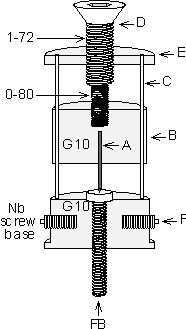
\includegraphics[width=0.5\linewidth]{images/JOS5.png}} \\
    Figure \ref{fig:JunctionAssemblyDiagram} (again): Junction Assembly
\end{center}

Two tiny set screws (F), which are not on opposite ends of the diameter, hold the junction in the probe. To remove the junction, one of the set screws must be turned \emph{in} (clockwise) to the fiberglass housing, so that it will clear the holes in the stainless steel tubing. Using an allen head wrench, gently turn the set screw clockwise until it clears. Check to see that the wire leads are free at the upper end of the probe, (i.e., the rubber cork should be out). Then gently pull the junction out of the tube. A slight twisting action helps.

When reinstalling the assembly, the crucial point is that there should be no resistance to backing out the set screw. The hole must be lined up exactly and the set screw backed out only far enough to hold the junction in place. No attempt should be made to tighten it.

\subsection{Installing a point in the assembly}

There are many tiny parts (screws, etc.) in this assembly that can be easily lost or damaged. When disassembling the apparatus, please do it directly over a clutter-free bench top, so that when the little parts do fall, they don't make it to floor to roll around and get lost. Get a container in which to put the parts. Take all the disassembled parts and store them in a safe spot where you will be able to find them when you are ready to reassemble the apparatus. Use a minimum of force and don't be afraid to ask for help if anything seems stuck.

To install a new point, you will have to first remove the existing one.

\noindent Steps to remove the old point:

\begin{enumerate}
    \item First back off the differential screw (D) until it comes out of the housing.

    \item Loosen the nuts associated with the screws (See Figures \ref{fig:JunctionAssembly} and Figure \ref{fig:DetailsOfPointHolderConstruction}) which have solder lugs attached to them, in piece (G10). You usually don't need to remove the nuts entirely (and its easier if you don't).

    \item Using small needle-nose pliers, gently pull the needle out of the housing (B).  You can prevent the screws from falling off by placing two fingers on opposite sides of the assembly applying a slight amount of pressure on the screws with each finger to still be able to remove the old point. Keep your fingers held in place with your fingers until you install the new point. If the screws come off, worry not, instructions on how to install them back and  fast will be provided to you below. Do this over a clean surface because the screws will probably fall out as you remove the needle.

    \item Throw the old needle away.

\end{enumerate}

\noindent Steps to install the new point when screws still in place:

\begin{enumerate}
    \item Use emery paper (or light sand paper) to remove the oxide layer from the \emph{back end }of the point (the last 3/8" or so), where it will meet the electrical contacts. Be careful you don't disturb the oxide layer on the tip of the point.

    \item Thread the new point through the lower screw shaft, making sure the solder lug corresponding to P1 is properly attached (see Figure \ref{fig:DetailsOfPointHolderConstruction}; note that the wires are color coded).

    \item Then thread the point through the upper screw shaft, with the lug for P2 properly secured. Tighten the nuts tight enough to make good electrical and mechanical contact, but not too tight. Too much tightening will bend the needle making it nearly impossible to remove. While holding the point close to the Nb base, but not touching it, replace the differential screw. Be careful that the tip of the differential screw does not touch the back end of the niobium needle, inadvertently grounding it. When the junction assembly is inserted into the tube, the screws and solder lugs may come in contact with the tube's inner wall, shorting them; it may be desirable to place insulating material, such as small strips of electrical tape, over these exposed connections (don't use very much; in the tube, space is limited)

\end{enumerate}

\noindent OR

\noindent Steps to install the new point when screws fell off:

\begin{enumerate}
    \item Use emery paper (or light sand paper) to remove the oxide layer from the \emph{back end }of the point (the last 3/8" or so), where it will meet the electrical contacts. Be careful you don't disturb the oxide layer on the tip of the point.

    \item Grab your new point with the black pliers, this will provide with a better grip, but make sure not to squeeze it too hard. Then insert the point through the same whole in the assembly until you reach the point before lower hole for the P1 screw.

    \item Pick up one of the screws and adjust the nut just enough so the screw barely clears the hole in the nut, this is approximately the length necessary to match the level at which the point will be threading through the hole in the middle of the screws. Do the same for the other screw.

    \item Choose either screw and align the hole axis with the point and insert the screw in the aperture for the lower screw P1 (you need not to hook your cables just yet). While holding the screw in place so it won't move out of alignment, use your other hand to grab the pliers and thread your point through the hole in the screw until it reaches the point before the upper screw aperture. If aligned properly or close to alignment the point will make its way through the point, otherwise if after a couple of tries it doesn't go through you may have to adjust the level of the whole a little; you can do this loosening your nut just a little so it will be just below the point the screw clears the whole aperture of the nut. (Do this with the other screw as well)  Repeat step 4 again until you are able to thread the point.

    \item Pick up the last screw and do the same thing as in step 4 but this time for the upper screw. Be careful that the tip of the differential screw does not touch the back end of the niobium needle, inadvertently grounding it.

    \item Now that the screws and point are in place start by loosening the lower screw nut and attaching the cable with the soldered lug corresponding to P1 and tighten back the nut after (Note that the wires are color coded and labeled at the top of the probe). Do the same for the upper screw which correspond to P2. Make sure your lugs are tight enough so they won't wiggle around. When the junction assembly is inserted into the tube, the screws and solder lugs may come in contact with the tube's inner wall, shorting them; it may be desirable to place insulating material, such as small strips of electrical tape, over these exposed connections (don't use very much; in the tube, space is limited).

\end{enumerate}

Replace the junction assembly in the probe tube. As you do this, make sure that the socket in the top of the differential screw mates securely with the drive shaft running the length of the probe. It also helps to have your partner gently take up the slack that develops in the wires as you move the assembly into the probe. Secure the assembly by backing out the retaining set-screw.

After you get everything hooked up, be careful with the probe; lay it flat on the table when its not in the cryostat (you don't want to loose all your hard work to a drop or a kick).

\begin{figure}[h]
    \centering
    \href{http://experimentationlab.berkeley.edu/sites/default/files/images/250px-JOS13.gif}{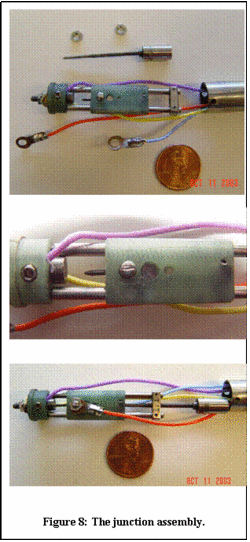
\includegraphics[width=0.3\linewidth]{images/250px-JOS13.png}}
    \caption{The Junction Assembly}
    \label{fig:JunctionAssembly}
\end{figure}

\subsection{Check for proper electrical continuity}

After installing the junction in the probe, check to see that an infinite resistance separates each output (B1, B2, P1, and P2) from ground (the metal body of the probe tube). B1-B2 as well as P1-P2 should show continuity. With an open junction, P1-B1, P2-B1, P1-B2, P2-B2 should show infinite resistance. You should do these checks before \emph{every} immersion in liquid helium.

\begin{figure}[h]
    \centering
    \href{http://experimentationlab.berkeley.edu/sites/default/files/images/JOS14.gif}{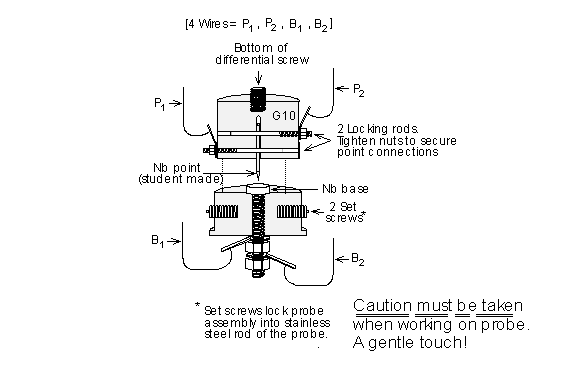
\includegraphics[width=0.5\linewidth]{images/JOS14.png}}
    \caption{Details of Point Holder Construction}
    \label{fig:DetailsOfPointHolderConstruction}
\end{figure}

\subsection{Make contact between the point and the base}

Connect an analog Ohm meter (e.g., the 3478A Multimeter) between P1 and B1. Set it to a scale that would display 50 Ohms easily (You may have to mess with the range). It should show an open circuit. Slowly tighten the screw at the top of the probe. Don't over-tighten the screw or you will scrape off your oxide layer and have to start all over. After a few turns, the VOM ought to suddenly show a small resistance, approximately a few Ohms, or tens of Ohms. If you can't get this behavior your point may need to be replaced.

\subsection{Connect the probe to the \texorpdfstring{$I$-$V$}{I-V} curve electronics}

Connect the probe to the electronics box on the side of the power meter, here you will see 4 connections. Follow the diagram in Figure \ref{fig:ElectronicsBlockDiagram} to properly connect the current oscillator, preamp, scope, P1, B1, P2, B2 to the probe. Good initial settings for the electronics are...

\begin{itemize}
    \item Scope: Set the scope for X-Y mode with 1 V/division for both axes and DC coupling.

    \item Low-frequency oscillator: Frequency = 60 Hz, Amplitude = $\sim$5 to 8 Volts peak-to-peak (so that the trace fills the vertical scale).

    \item Preamp: Gain = 500, Bandwidth 0.03 Hz - 30 KHz, DC coupling for both channels.
\end{itemize}

You should see a straight line on the scope with the preamp turned off. You may have to play with a number of the above settings; every point is different. The Low-Frequency oscillator is set to 60 Hz to match any 60 cycle pick up, but the wall current may vary (20 mHz, so you may need to adjust the frequency slightly to get a signal on the scope that doesn't oscillate. By using the slope of the $I$-$V$ line, calculate the room-temperature resistance of the junction. It should be the same as what you measured on the VOM.

\textbf{This is a checkpoint and a great time to stop and think about the physics at play. Discuss the following questions with you partner and once you feel you have a better understanding of what is happening, call over a GSI to sign you off:}\\
Will matching the Low-Frequency oscillator to the wall current frequency affect the conclusions you will be drawing? What systematic error could occur?

\subsection{Before you Insert the probe into the cryostat}

Liquid helium is expensive. So you must be careful in order not to waste it. As mentioned, each time you go to cool the probe, you should check for shorts, proper continuity, and proper junction resistance. Only if everything checks out and is working properly, may you proceed to insert the probe into the cryostat. You should only need to immerse each point once. As most of the helium boil-off occurs with the cool down, it is the number of immersions, not the length of time the sample is immersed, that will determine how much LHe is used.

Liquid helium has a low heat capacity. So you must be gentle when handling the cryostat. You can boil off a lot of extra helium just by shaking the cryostat or making excess turbulence inside it. To avoid excessive boil off during insertion, it is useful to know how much LHe is in the cryostat.Follow safety precautions before starting handling this cryogenic liquid (He). You will want to first check the pressure in the tank is marking around zero, if this is not the case then check if the flow valve directly position opposite to the pressure valve (180 degrees) is open; if not contact Don Orlando or a professor immediately. This valve regulates the pressure of the tank and should always be kept open!. If the pressure is close to zero then you shall proceed. Open the valve at the top of the cryostat. It will vent for a few seconds. There should be a long, thin ($<$ 1 cm) metal tube with a latex membrane over one end located at your station. Hold a finger over the membrane and lower the tube into the cryostat; note when it touches the bottom. As LHe boils off, He vapor traveling up the tube should cause the membrane to vibrate. Lift the tube and note its height when you feel the vibration change; this gives you the depth of the LHe.

Before you cool the probe, check that it is completely dry; any leftover condensation from previous cooling cycles on the exterior of the probe could quickly form dangerous, neck clogging ice, while and liquid in the point assembly could ruin the experiment. Remove all the electrical connections from the probe, and check that the rubber plug (R) and RF coupling port cap are securely in place.

Carefully insert the probe into the cryostat, turning it back and forth as you go to prevent sticking. When the probe is an inch above the surface to the LHe, as you measured it, slow up its descent. Helium will rush out past the sides of the probe as you immerse it. Don't go too fast. The sound of the rushing helium should be soft and quiet, if it gets too loud (if you can hear it above the din in the 111-lab, it probably is) stop lowering the probe until it subsides, \emph{but don't stop turning it}. The probe is more likely to freeze to the cryostat during excessive outflow. If the probe freezes into the storage vessel neck such that it cannot be turned or removed, call a staff member \emph{immediately}. This is potentially quite dangerous as pressure in the vessel could build up.

Every day, before you go home, you should remove the probe from the cryostat; if the probe is left unattended overnight, the neck could freeze closed and there could be an explosion. You should make sure you close the cryostat valve after the probe is removed to avoid wasting LHe. Whenever the probe is taken out of the liquid helium, it should be dried. There is a heat gun on the lab table; use it to remove any condensation and heat the entire probe, including the point assembly, until it is warm to the touch (not hot: you don't want to melt anything). Even if you are leaving the probe overnight, it is important to dry it, as you some condensed water may not evaporate.


\textbf{This is a checkpoint and a great time to stop and think about the physics at play. Discuss the following questions with you partner and once you feel you have a better understanding of what is happening, call over a GSI to sign you off:}\\
Explain the steps and why you must follow these instructions before inserting the probe into the cryostat, when lowering the probe down the cryostat, and after the probe has been removed.

\subsection{Observe the DC effect}

\begin{figure}[h]
    \centering
    \href{http://experimentationlab.berkeley.edu/sites/default/files/images/250px-JOS15.gif}{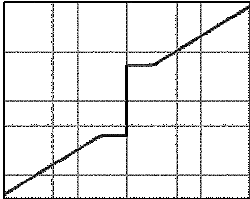
\includegraphics[width=0.5\linewidth]{images/250px-JOS15.png}}
    \caption{$I$-$V$ curve of DC effect}
    \label{fig:IVCurveOfDCEffect}
\end{figure}

Connect the probe outputs to the electronics and observe the $I$-$V$ curve displayed on the scope. Gently turn the screw to obtain the DC effect. You may very quickly see an $I$-$V$ curve that looks like the DC effect (see Figure \ref{fig:IVCurveOfDCEffect}). Test whether this is a true DC Josephson effect or a supershort by bringing the large permanent magnet near the cryostat. If you have the DC effect, you should see fluctuations in the maximum current that flows without a voltage drop as you move the magnet around. If you do not observe these fluctuations, keep adjusting. You should find that the DC Effect is not too difficult to get, although it takes patience. If you don't get a good effect, try subtly raising and lowering the point with the screw; each time you do this, you make the contact at a slightly different location (were talking Angstroms here) with potentially different properties at the same time, with each contact, some of the oxide layer is removed (which may or may not be a good thing).

First you should use the analog scope to see all of your data DC and AC effects, then use the Josephson junction VI accessible from the desktop to acquire more data (This is a LabView program). You will have to switch your leads from the oscilloscope to the DAQ on your work station table. Once you open your JSO LabView program  on the top tab you can select the input ports where you will now connect your leads. You should be saving your data collected.

\textbf{This is a checkpoint and a great time to stop and think about the physics at play. Discuss the following questions with you partner and once you feel you have a better understanding of what is happening, call over a GSI to sign you off:}\\
Did you observe decent results of DC effect on the scope? What changes did you made in order to improve your observation?

\subsection{Observe the AC effect}

Once you have a good DC effect, you are ready to get the AC effect by applying the microwaves. First turn on the RF Oscillator (Figure 11) and the Microwaves doubler power supply. Then measure the RF power. Set the attenuator to 20 dB, then attach the power meter to the waveguide \href{http://experimentationlab.berkeley.edu/sites/default/files/JOS/waveguide.jpeg}{\textbf{like this}} (You may have to unscrew the waveguide connection to the probe before). Set the \href{http://experimentationlab.berkeley.edu/sites/default/files/JOS/image.jpeg}{\textbf{power meter}}'s scale to 10 mW and the mount resistance to 200 Ohms (We do this merely to make sure there is power coming out of the waveguide, don't spend too much time here). You must keep the attenuation at a value that gives a power reading without overloading the meter. The thermistor detector, connected to the waveguide, may be damaged if you apply it more than 15 mW power (15mW maximum), so be careful. That is why the microwave attenuator is set to 20dB to start.

You will vary the RF source to a frequency in the 9 - 13 GHz range( this is sent to the frequency doubler to get 18-26 Ghz). A good place to start is around the middle of the range by pressing the ``CW'' button followed by the frequency on the Data Entry pad press\textbf{ 1, 1, GHz} for 11 GHz (It is usually set to this value when the RF Oscillator is turned on). The display should look like the picture below (Figure 11). You can adjust the frequency with the knob below the display, and it's a good idea to do so when you search for the AC effect.

\begin{figure}[h]
    \centering
    \href{http://experimentationlab.berkeley.edu/sites/default/files/images/JOS16.jpg}{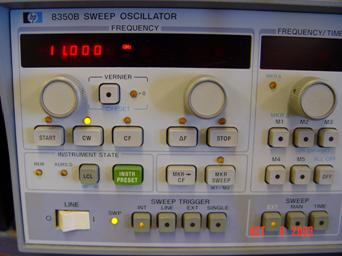
\includegraphics[width=0.4\linewidth]{images/JOS16.jpg}}
    \caption{RF Oscillator}
    \label{fig:RFOscillator}
\end{figure}

Because the doubler doesn't precisely double the frequency of the RF Oscillator, practice measuring the output frequency by tuning the absorption cavity. Start by tuning the absorption cavity in the neighborhood of twice the displayed frequency of the RF source. Probe the crystal detector with the oscilloscope in channel 1 and set it to DC mode; you should see a line on the scope if triggered correctly. Once you get a steady DC voltage you can start varying  the cavity. When you observe the highest increase in the DC signal, the cavity is tuned to the RF frequency, which may be read off of the cavity's scale (finding the cavity requires a finite tuning due to the small signal, proceed slowly). If you have trouble finding the RF frequency you can also feed your signal the Pre-Amp to amplify it by setting it to DC coupling, SOURCE A, not filter cutoffs, and a gain of 100.

The RF system will generate about 50 to 350 mW of power (The power can be more and that's okay). Record how much power you're getting (based on the power meter readings and the attenuation, as well as the frequency). Then connect the waveguide to the probe.

To find the AC effect, you really only have three variables at your disposal: RF power, RF frequency, and junction pressure. To vary the power, either use the attenuator, or the power output knob on the RF source (the former is probably best). Tweak the pressure of the point contact as you watch for faint steps. Most probably you will need to vary the microwave power and the pre-amp / scope settings to see the effect. The best advice is to play with everything at your disposal to obtain the effect. When you have as many clear steps as you can find, take a photo of the scope display for analysis. The AC effect is a little more difficult to achieve, but everyone does get it after some adjustments; have patience and be gentle. Once you have the AC effect, leave the RF frequency set-up undisturbed; you will want to make a precise frequency measurement after you have calibrated the PRE-AMP and scope.

First you should use the analog scope to see all of your data DC and AC effects.

\begin{figure}[h]
    \centering
    \href{http://experimentationlab.berkeley.edu/sites/default/files/images/250px-JOS17.gif}{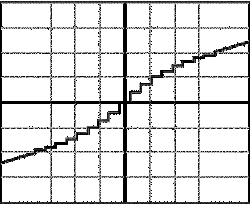
\includegraphics[width=0.5\linewidth]{images/250px-JOS17.png}}
    \caption{$I$-$V$ curve of AC effect}
    \label{fig:IVCurveOfACEffect}
\end{figure}


\textbf{This is a checkpoint and a great time to stop and think about the physics at play. Discuss the following questions with you partner and once you feel you have a better understanding of what is happening, call over a GSI to sign you off:}\\
\subsection{Calibration}

As you might imagine, the accuracy of your results depends critically on the calibration of the voltage axis of the $I$-$V$ curve. One method of calibration would be to measure the gain of each individual piece of the signal chain (junction to pre-amp to scope) and multiply them together. But that becomes impractical as the number of signal chain elements grows, and is more prone to error than the alternative. So, although the signal chain in this experiment is not too complex, you are going to use the technique of measuring end-to-end gain. Replace the Josephson junction, two wire cables, with a voltage box about 517 µV. Measure the box voltage with the DVM and hook it up to replace the point contact voltage. Measure the limits of the excursion of the trace on the scope and use this to calibrate your equipment setup. See pictures below.

\noindent
\begin{minipage}[t]{0.5\linewidth}
    \centering
    \href{http://experimentationlab.berkeley.edu/sites/default/files/JOS/Voltage-Ref_4058.JPG}{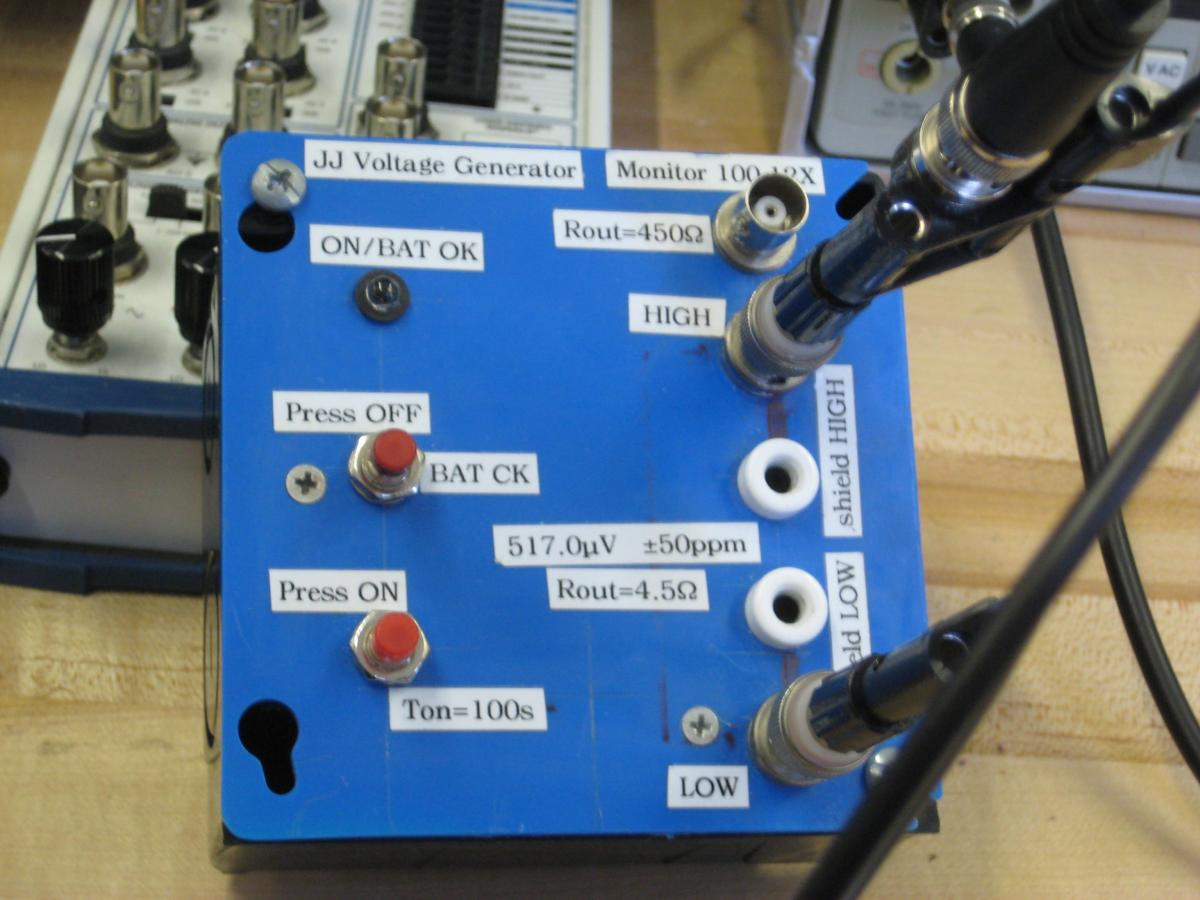
\includegraphics[width=\linewidth,keepaspectratio]{images/Voltage-Ref_4058.JPG}} \\
    Voltage Reference Box 517 $\mu$Volts \\\vspace{1em}
    \href{http://experimentationlab.berkeley.edu/sites/default/files/JOS/V-Ref-Setup-0_4060.JPG}{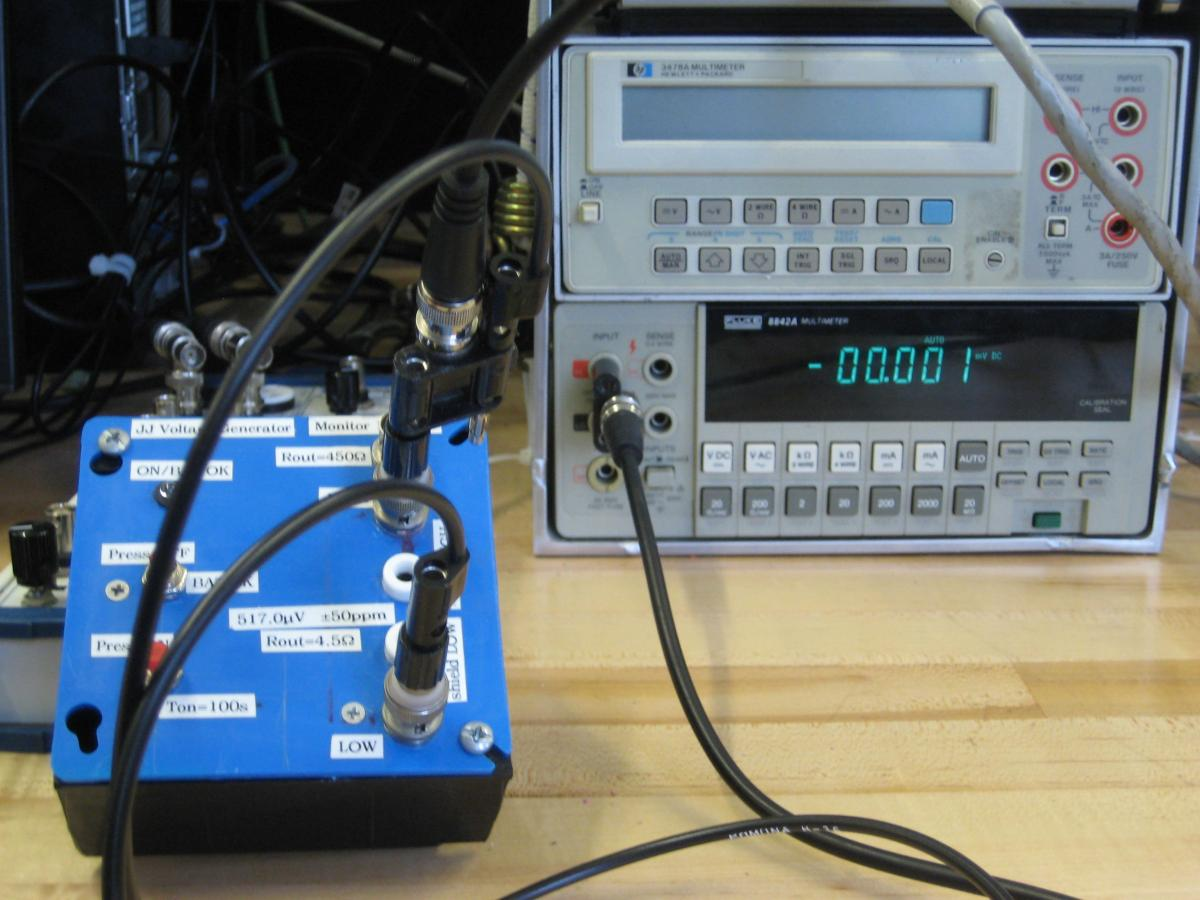
\includegraphics[width=\linewidth,keepaspectratio]{images/V-Ref-Setup-0_4060.JPG}} \\
    Zero Reference on Meter - Note zero
\end{minipage}
\begin{minipage}[t]{0.5\linewidth}
    \centering
    \href{http://experimentationlab.berkeley.edu/sites/default/files/JOS/V-Ref-Hookup_4055.JPG}{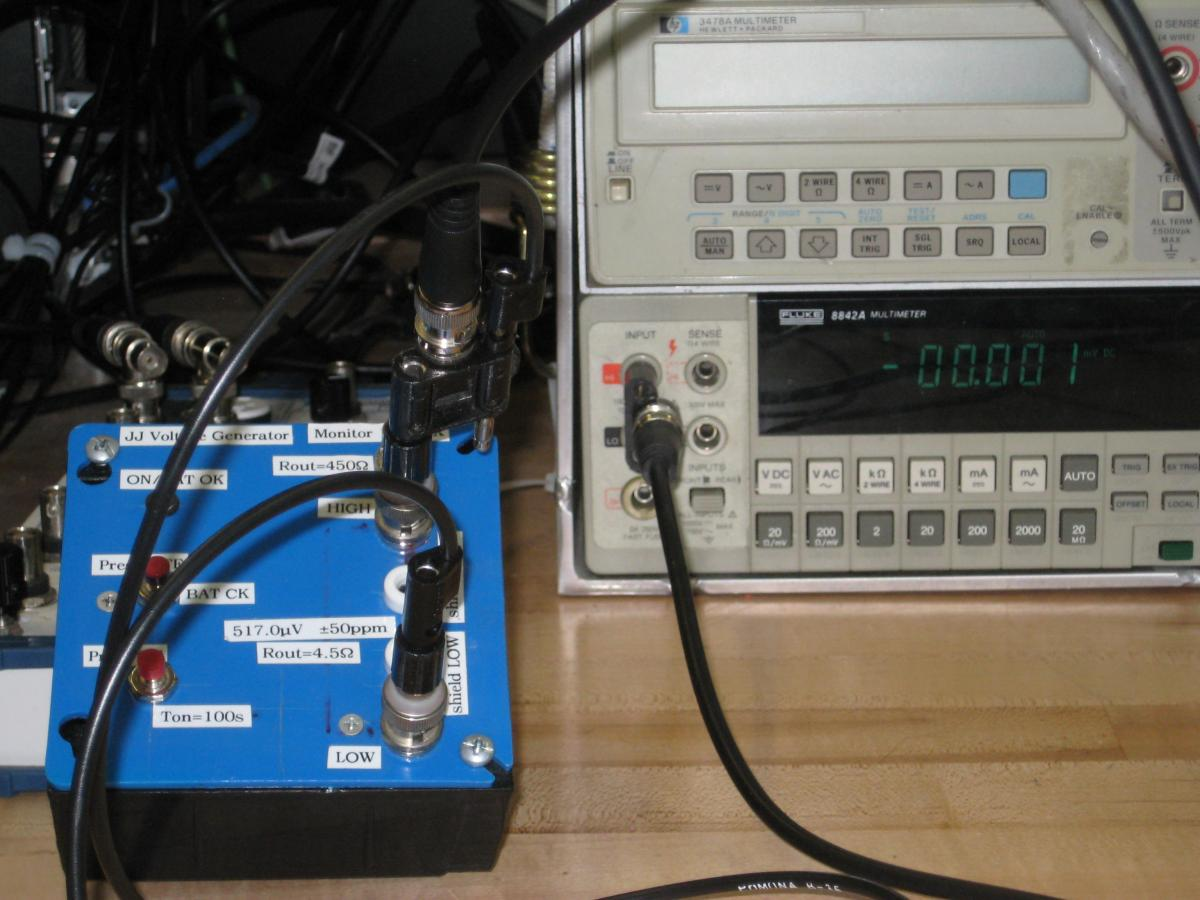
\includegraphics[width=\linewidth,keepaspectratio]{images/V-Ref-Hookup_4055.JPG}} \\
    Voltage Reference Hookup \\\vspace{1em}
    \href{http://experimentationlab.berkeley.edu/sites/default/files/JOS/V-Ref_setup-517uV_4061.JPG}{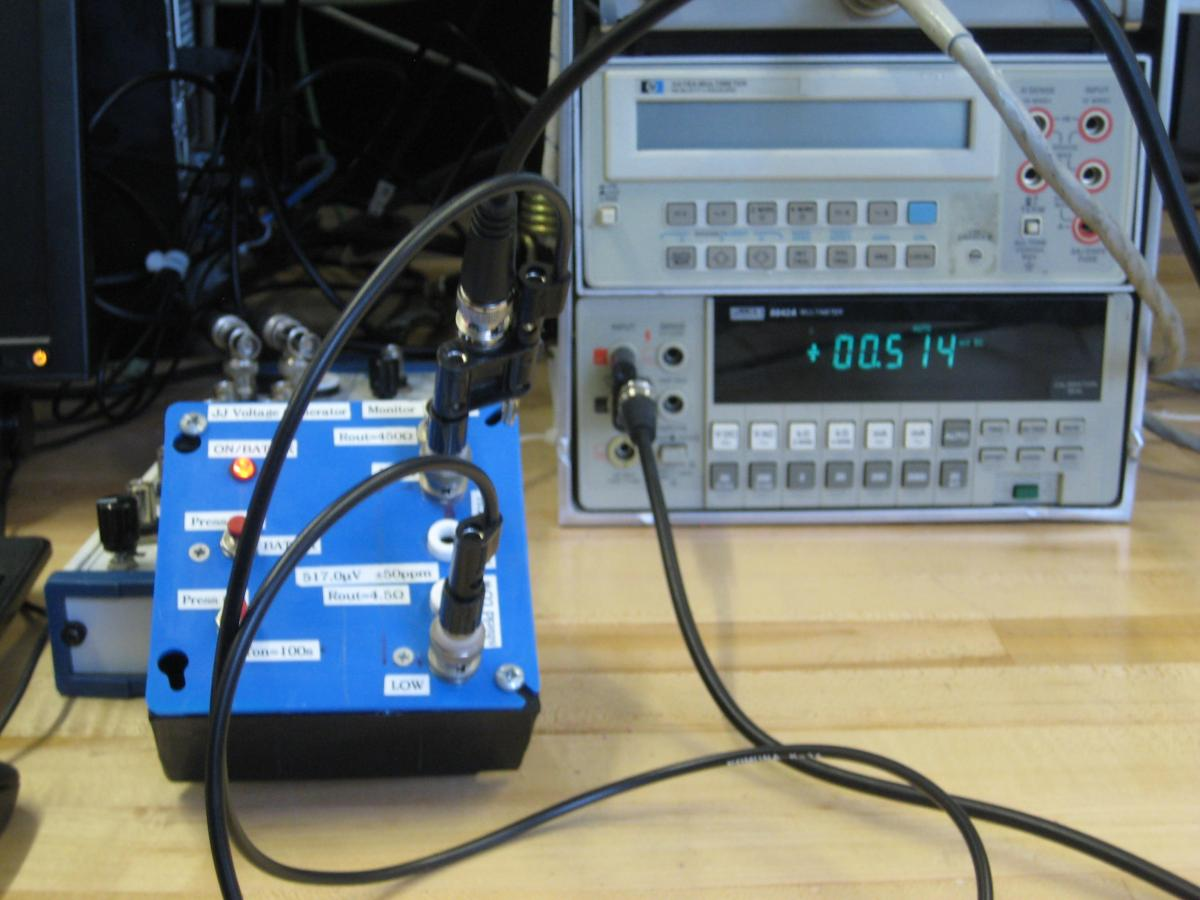
\includegraphics[width=\linewidth,keepaspectratio]{images/V-Ref_setup-517uV_4061.JPG}} \\
    Read voltage on Meter + zero reading
\end{minipage}

\vspace{1em}

\noindent Specifically:

\begin{itemize}
    \item Determine the number of divisions that the dot spans on the scope.

    \item Using the digital volt-meter (DVM)at the lab setup, measure the RMS amplitude of the signal that you are applying to the pre-amp.
\end{itemize}

Be sure to record estimates of your measurement uncertainties. Calculate the end to end gain.

Make a precise measurement of the RF frequency using the absorption cavity and make an estimate of 2$e/h$. What do you trust more the synthesizer reading or the cavity measurement? As with all experiments, you should be calculating and checking results in lab, as you go through the experiment. Don't take data and expect that it will all work out later.

\section{Report}

\begin{enumerate}
    \item Be sure that your report includes the oscilloscope pictures with the axes \emph{clearly labeled} and \emph{scaled for} quick identification.

    \item Compare your value for 2$e/h$ with that obtained by Parker, Taylor and Langenberg \href{http://physics111.lib.berkeley.edu/Physics111/Reprints/JOS/04-The\_Josephson\_Effects.pdf}{\textbf{The Josephson Effects}} (Phys. Rev. Letters 18, 287 (1967)) of (483.5912 + 0.0012) MHz/microvolt. Explain any major discrepancies between your results and theirs. What are the errors on your measurements? Are your errors consistent with the quality of your data?

    \item When displaying the $I$-$V$ characteristic, which of the axes needs high band-width. Why do we not need high band-with for the other axis?

    \item What physical significance does an accurate measurement of the ratio e/h have?

    \item What do the microwaves do in this experiment?

    \item Why not use another frequency range like 100 MHz?

    \item Last day of the experiment please fill out the \href{\ExperimentEvaluation}{\textbf{Experiment Evaluation}}

\end{enumerate}

\section{References}
\label{sec:References}

\begin{enumerate}
    \item Richards, P.L. ``\href{http://physics111.lib.berkeley.edu/Physics111/Reprints/JOS/06-The\_Josephson\_Junction\_as\_a\_Detector.pdf}{\textbf{The Josephson Junction as a Detector of Microwave and Far Infrared Radiation}}''; UCRL-19035, Lawrence Radiation Lab, pp. 1-35.

    \item Maglich B. ``\href{http://physics111.lib.berkeley.edu/Physics111/Reprints/JOS/09-Observation\_of\_Josephson\_Effect.pdf}{\textbf{Observation of Josephson Effect and Measurement of e/h}},'' Adventures in Experimental Physics - gamma volume, Chapter 2.

    \item Kittel, Charles. ``\href{http://physics111.lib.berkeley.edu/Physics111/Reprints/JOS/JOS\_Introduction\%20to\%20the\%20solid\%20state\%20physics.pdf}{\textbf{Josephson Superconductor Tunneling Effect}}.'' \emph{Introduction to Solid State Physics}. Third ed. New York: John Wiley and Sons, 1969. Pp. 737-743.

    \item Eisberg, R. and Resnick R. "\href{http://physics111.lib.berkeley.edu/Physics111/Reprints/JOS/Semiconductors\%20&\%20Magnetic\%20Prop.\%20Ch-14-pg.\%20532.pdf}{\textbf{Ch. 14: Solids -- Superconductors and Magnetic Properties}}.” \emph{Quantum Physics of Atoms, Molecules, Solids, Nuclei, and Particles}. Pp 532. New York: John Wiley and Sons, 1974.

    \item Taylor, Pointon ``\href{http://physics111.lib.berkeley.edu/Physics111/Reprints/JOS/07-Microwave\_Ultrasonics.pdf}{\textbf{Microwave Ultrasonics}}''; Contemporary Physics, Vol. 10, No.2, 1969, pp 159-178

\end{enumerate}

\noindent Other reprints and reference materials can be found on the \href{http://physics111.lib.berkeley.edu/Physics111/Reprints/JOS/JOS\_index.html}{\textbf{Physics 111 Library Site}}

\end{document}
